\chapter{Results}

Performing optimal control of quantum many-body systems is typically extremely resource demanding \cite{Mennemann2015}. Hence, previous studies of optimization of Bose-Hubbard dynamics have abstained from using gradient-based techniques and instead opted for the gradient-free Nelder-Mead method combined with control parameterizations \cite{Doria2011,FrankBloch}. The framework presented in this thesis combines tensor description of lattice systems with parameterized optimal control methods and highly-developed gradient-based algorithms from mathematical optimization theory. Here, the framework is used for optimizing the ramp sequence for transitioning from a superfluid to a Mott-Insulator in a Bose-Hubbard system, however, the method can easily be extended to any system in a one-dimensional lattice.
Although the individual components of the framework are described in previous chapters, a summary of their unification is brought here:

The physical quantum system is represented using Matrix Product States described in Chapter \ref{chap:MPS}. Through the many Schmidt decompositions used for creating and modifying the tensor networks weakly contributing eigenstates are discarded, whereby one avoids the otherwise exponential scaling of the numerical representation with physical size of the system. For the purposes of this thesis, the ITensor library \cite{ITensor} has proven itself very useful for tensor-operations.
To simulate the dynamics of the system, a modified version of the tDMRG algorithm described in Section \ref{sec:modTMDRG} is employed. The algorithm efficiently time-evolves the tensor network states while maintaining an accurate description of the system.
In order to address the crossing of the phase transition in the Bose-Hubbard model, the state transfer is formulated as the minimization of a cost function \eqref{eq:grapeCost} through the optimal control framework of Chapter \ref{chap:OptimalControl}. The GRAPE method supplies derivatives of the cost function with respect to the control parameters \eqref{eq:STcostgrad}, whereby the optimization problem can be solved using gradient-based techniques. Further extensions are added through GROUP, which parametrizes the control through smooth functions \eqref{eq:controlParametrization} thereby reducing the dimension of the optimization space.
Due to limits of the physical model, the control problem is subjected to a series of constraints, which makes the optimization very difficult. 
Interior Point methods are considered some of the most powerful algorithms for solving non-linear, constrained problems. Using the gradient of the cost function, the algorithm approaches the optimal control values from within the feasible region. Thus, interior point methods require fewer, but more expensive, steps to converge, which is a beneficial feature when using the computationally expensive GRAPE gradient. The version of the Interior Point method used here is implemented in IPOPT library \cite{Wachter2006}.\\

In this chapter the performance and accuracy of the framework is analyzed. First, suitable optimization settings and boundary conditions are discussed.
Next, the framework is applied to a small Bose-Hubbard system of five sites and five particles, and its performance is compared to optimizations performed using the Nelder-Mead method.
Finally, the application of the framework on larger systems is discussed, and an analysis of the entanglement entropy during quenches past the critical point is made. 


\section{Determining Optimization Parameters}

As previously discussed in section \ref{sec:modTMDRG} the phase of Bose-Hubbard model is solely determined by the fraction $U/J$. Expressing the parameters in units of $J$, causes the tunneling part of the Hamiltonian to act as a drift, while the interaction matrix element, $U$, serves as the control function.\\
The time evolution is carried out using Suzuki-Trotter decomposed propagator, where the Trotter step has been chosen as $\Delta t = 10^{-2}$. The Trotter step is larger than in other studies \cite{Doria2011,FrankBloch,Braun2015}, however, any smaller step-size would result in numerical costs outside the scope of this thesis.


\subsection{Boundary Conditions and Constraints}
The Bose-Hubbard model is only well defined within the tight-binding limit. Below this limit the Wannier functions may start overlapping with the next-nearest neighbouring sites thereby facilitating two-site hopping, which is not accounted for in the model. Thus, the control function must be subjected to a lower boundary. In \cite{FrankBloch,Doria2011} initial lattice depths at $V_0 (0) = 3 E_{\mathrm{rec}}$ and $2 E_{\mathrm{rec}}$ were chosen, where it was argued that the model is still a decent approximation at this depth.
Taking a conservative approach, the control here is subjected to the constraint $U (t) \geq 2 J$, which corresponds to a lattice depth around three recoil energies for a gas of Rb-87 atoms and an optical lattice with wavelength $\lambda = 1064 \: \mathrm{nm}$. 
The initial control value was set slightly above the minimum value at $U (0) = 2.5 J$. Initially, the first control value was chosen to be equal to the lower bound, however, initiating the interior point algorithm at the edge of the feasible region caused to method to exhibit a poor convergence rate during its initial cycles.
The final control value was set to $U (T) = 50 J$, which roughly corresponds to the final lattice depth of $V_0 (T) = 14 E_{\mathrm{rec}}$ used in \cite{FrankBloch}.\\
The initial and target state were calculated from the control parameter at the start and end of the duration respectively using the DMRG algorithm. Thus, the states are insured to be the ground state at each end of the duration, whereby the optimized state transfer will bring be between two ground states.


\subsection{Seed Selection}
The success of an optimization process is often dependent on the quality of the initial starting point or seed. Poor seeding strategies can lead to failure in finding optimal solutions when conducting local searches in complex optimization landscapes \cite{Sorensen2016}. This has been demonstrated to occur in constrained quantum control problems \cite{Zhdanov2015}. Hence, the type of seed used for the optimization must be chosen carefully.\\ 
Different adiabatic lattice ramps from the superfluid to Mott-Insulator phase were examined in \cite{Zakrzewski2009}. The study concluded that ramping the lattice slowly around the point of the phase transition results in an improved final fidelity, which is very similar to the process of sweeping over an avoided crossing \cite{manybodyBloch}.\\
Therefore, a ramp sequence was proposed in \cite{Zakrzewski2009}, which has an initial sigmoid shape followed by a slow increase in the lattice depth around the phase transition point. Following this, the lattice follows an exponential ramp to its final depth. Examining other attempts of optimizing the ramp sequence of the Bose-Hubbard model \cite{Doria2011,FrankBloch} shows similar traits in their results. Therefore, choosing seeds with a slow ramp across the point of the phase transition followed by a rapid increase in lattice depth should yield good optimization results.
\begin{figure}[h!]
    \centering
    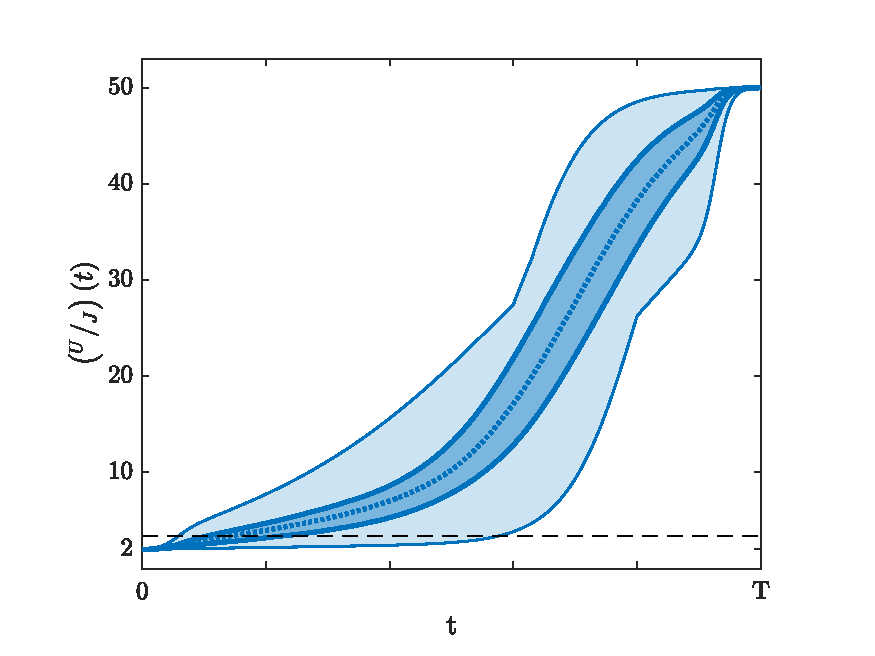
\includegraphics[width=0.7\textwidth]{Figures/LinSigSeed.pdf}
    \caption{\textit{Distribution of seeds used for optimization. All seeds lie within the lightly shaded region, while the darker region contains the 25-75 percentile of seeds. Lastly, the dotted line is the median value of the seed. The dashed line signifies the point of the Bose-Hubbard phase transition.}}
    \label{fig:LinSigSeed}
\end{figure}
Figure \ref{fig:LinSigSeed} shows the distribution of seeds used for the optimizations. Due to control parameter being the interaction strength of the Bose-Hubbard model, the phase transition occurs at quite a low control value. Hence, the initial part of the seed is a slowly increasing linear ramp, which crosses the point of the phase transition with a small slope. A shape function has been multiplied to the seeds enforcing a horizontal slope at the start and end of the duration, which helps avoiding any kinks in the control curve.



\section{Optimization of Dynamics in 5-Site Lattice} \label{sec:5partOptimization}
Previous studies of ramp sequences for the superfluid to Mott-insulator have employed the gradient-free Nelder-Mead optimization method \cite{Doria2011,FrankBloch}. Thus, to illustrate the power of interior point methods in non-linear and highly constrained problem, the same optimization problem was solved using both Nelder-Mead and interior point methods. While the framework is designed to conduct optimizations on larger systems, for the comparison of these two methods a 5-site lattice system with unit occupancy will suffice. Due to the small size of the system, no maximum bond dimension was required. Instead, a truncation threshold of $\epsilon_t = 10^{-8}$ was used. Furthermore, the relative tolerance used by the IPOPT library for determining convergence was set at $\varepsilon_t = 10^{-8}$. The optimization was carried out using a tolerance of $\varepsilon_t = 10^{-7}$ as well, however, the higher tolerance did not cause any notable change in neither obtained fidelity nor convergence rate, whereby these results are omitted.
Lastly, a regularization factor of $\gamma = 10^{-6}$ was employed. Since the control is parametrized using a linear combination of smooth functions, the effect of the regularization term is limited. Nevertheless, it does help the optimization algorithm avoid greatly varying controls during its initial iterations.
 

\subsection{Determining the Quantum Speed Limit}
In order to determine the quantum speed limit, one must solve the optimization problem for a series of durations, as calculating the quantum speed limit is otherwise a formidable task. In a complex quantum system, unit fidelity is only obtainable at very long duration. Therefore, one must decide on a fidelity threshold at which the obtained final state is sufficiently close to the target state. When deciding on this threshold, one must consider the size of the systems, as high fidelities are generally harder to obtain for larger systems. In \cite{MajaJulie} a similar optimization was made for lattice system of 3 sites. There, an infidelity threshold of $I_{\mathrm{QSL}} = 10^{-3}$ was used, which will be adopted for this optimization.
Since the result of the optimization often depends on the initial guess, 50 optimizations were carried out using both Nelder-Mead and interior point methods. The seeds were drawn for the distribution of ramps shown in figure \ref{fig:LinSigSeed}. For the following calculations a chopped basis size of $M = 20$ was chosen.

Figure \ref{fig:FidelityDuration} shows the final fidelities obtained for the superfluid to Mott-insulator transfer in the 5-site Bose-Hubbard system. While both methods manage to produce high fidelities, the interior method is clearly consistently better at every duration.
\begin{figure}[h!]
    \centering
    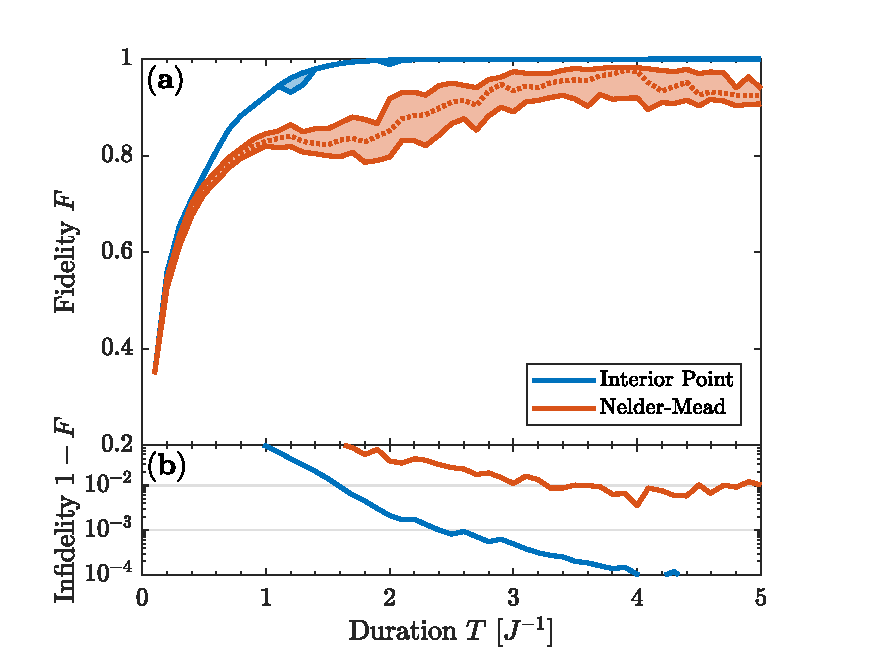
\includegraphics[width=0.9\textwidth]{Figures/L5/FidelityDuration.pdf}
    \caption{\textit{Final fidelity obtained for optimal control at various durations. \textbf{(a)} Median fidelity achieved marked by a dotted line, while the shaded area displays the $25\%$- and $75\%$-quartiles of the solutions. \textbf{(b)} The lowest infidelity achieved for each duration. }}
    \label{fig:FidelityDuration}
\end{figure}
In part \ref{fig:FidelityDuration}(a) the $25\%$- and $75\%$-quartiles along with the median of the solutions are displayed. At short durations the system can not evolve fast enough from the initial state to reach the target state, hence only low fidelities are obtained. The shortest duration of $T = 0.2 \; J^{-1}$ is almost a magnitude smaller than the time-scale of the tunneling. Therefore, the system can barely change from its initial configuration, whereby the different optimization methods produce identical results. However, as the system is given more time to evolve, the interior point method is much better at finding high-fidelity ramp sequences. Furthermore, the interior point method finds the optimal solution much more consistently, as the $25\%$- and $75\%$-quartiles of the solutions are almost indistinguishable from the median.

Information regarding the control landscape can be inferred from the variance in obtained fidelities. A small variance points towards a simple landscape with few local minima, while landscapes with many suboptimal solutions should produce a larger variance in obtained results. For short durations the system barely has time to change, whereby only very few solutions are possible. Therefore, the landscape is very simple, which is reflected in the extremely small variance produced by the interior point method. However, despite the simple landscape, the Nelder-Mead method converges to very different solutions. This is most likely due to the high convergence tolerance used for the Nelder-Mead optimizations, as only few improvements will be made for an already good starting guess. For comparison, a series of optimization were made using poor initial seeds for the Nelder-Mead method. Surprisingly, initiating the algorithm from an ill-behaving ramp actually caused it to converge towards the same solution as the interior point method. However, at longer durations, the optimizing using poor seeds led to considerably worse solutions as those displayed in figure \ref{fig:FidelityDuration}. Employing a lower tolerance should therefore result in better solutions achieved by the Nelder-Mead method, although this would significantly increase the number of function evaluations required for convergence. As shown in the next section, the Nelder-Mead method already has a very low convergence rate, whereby lowering its tolerance would severely lower its efficiency.

Figure \ref{fig:FidelityDuration}(b) displays the best solutions obtained for each duration. Plotting the result as an infidelity on a log scale clearly illustrates that the achieved fidelity continues to improve for longer durations. From the predetermined infidelity threshold, the quantum speed limit for the superfluid to Mott-insulator transition in a 5-site system can be inferred. Here, the interior point methods produces a quantum speed limit of $T_{\mathrm{QSL}}^{\mathrm{IP}} \sim 2.4 J^{-1}$ while it is $T_{\mathrm{QSL}}^{\mathrm{NM}} \sim 3.2 J^{-1}$ for the Nelder-Mead method. 
At long durations many optimal solutions exists, whereby the variance in results should be rather low. At durations on the order of $T \sim 5 J^{-1}$, the system has been evolved for timescales comparable to the tunneling time from one end of the lattice to the other. Thus, the duration is sufficient for the system to realize most of its possible configurations. Hence, both optimization algorithms should be capable of consistently finding high-fidelity solution, which is confirmed by the very low solution variance in figure \ref{fig:FidelityDuration}(a) for long durations. Meanwhile, for duration on the order of $T \sim 2 J^{-1}$  the evolution of the system is more restricted, whereby the impact of finding a good control sequence is larger. In fact, comparing the best solutions of figure \ref{fig:FidelityDuration}(b) reveals that the largest relative difference in obtained infidelity between the two methods occurs for these medium-long durations.\\

Previous optimizations of the superfluid to Mott-insulator phase have employed alternative figures of merit to the fidelity \cite{Doria2011,FrankBloch}. There, a rescaled variance of the particle number in each of the central sites of the lattice was employed. Although this figure of merit is less sensitive to system size than the fidelity, it does have some less favorable properties: First, multiple particle configurations different from unit occupancy of each site can achieve a vanishing particle number variance. Furthermore, the pure state of a single particle on each lattice site only becomes the ground state as the lattice depth tends towards infinity. Therefore, the number-variance figure of merit does not steer the state towards the ground state at the final control value, which will result in residual oscillations of the system after the control sequence. Therefore, the fidelity is a much better choice of figure of merit for the purpose of a state transfer to the ground state at a given control value.


\subsection{Convergence Rate}
Although obtaining a high fidelity is an impressive feat, most optimization algorithms should be capable of achieving high fidelities if a low enough convergence tolerance is employed. However, choosing a too high convergence tolerance will result in the algorithm running for long periods of time while only achieving minor improvements to the result. Therefore, it is important to investigate the convergence rate of the different methods, as their efficiency is extremely important for applications on larger systems.
\begin{figure}[h!]
    \centering
    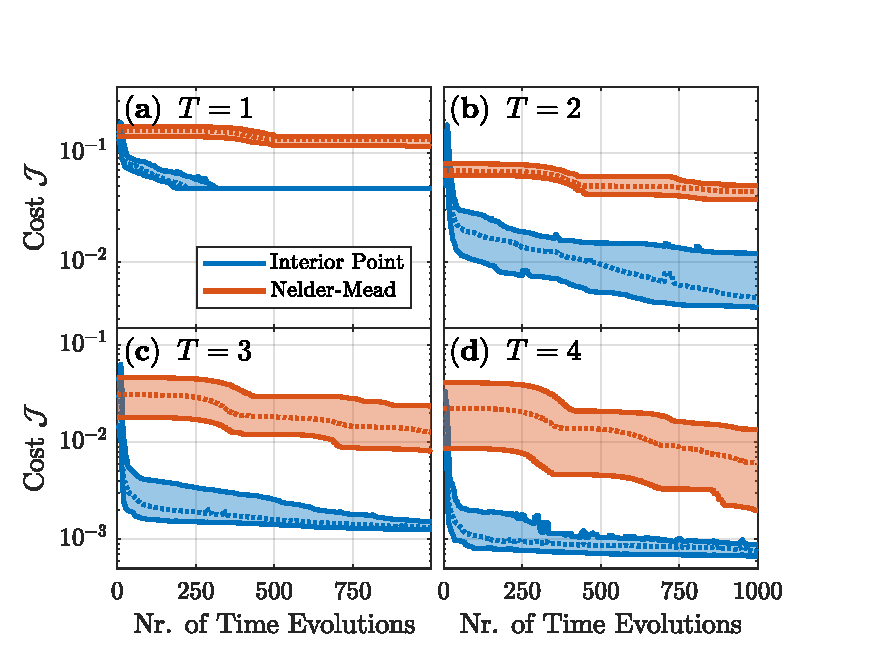
\includegraphics[width=0.9\textwidth]{Figures/L5/CostProgress.pdf}
    \caption{Optimization progress of the different optimization algorithms at various durations. The durations are in units of inverse tunneling strength. The dotted line marks the median cost \eqref{eq:grapeCost} at a given number of time evolution, while the shaded area illustrates the $25\%$- and $75\%$-quartiles of the current solutions.}
    \label{fig:CostProgress}
\end{figure}

The optimization process of the two algorithms tested is very different, as the Nelder-Mead method solely evaluates the cost function \eqref{eq:grapeCost}, while the interior point method requires both the gradient \eqref{eq:costGradient} to compute the step-direction and the cost function for a line search determining the step size. In both the computation of the cost and the gradient, the most resource-consuming calculations are the time evolutions of the state. Here, the computing the cost requires $N$ propagations of the initial state, while $2 N$ propagations are needed for evaluating the gradient. If the gradient and the cost are computed for the same control sequence, one only needs to propagate the initial state once thereby saving a full time evolution. For the interior point method, this will be the case for the first function evaluation in each iteration, however, each step of the line search will be done using a different control, whereby the initial state must be propagated anew.
Therefore, when comparing the convergence rate of the two methods, one should examine their obtained cost at a given number of time evaluations. Such a comparison is shown in figure \ref{fig:CostProgress} for a series of durations. Examining the progress of the two algorithms, one will notice that they behave quite differently. While starting at the same cost, the interior point method very quickly finds a control producing a much higher fidelity. This is possible through the gradient, which yields the optimal stepping direction for the optimization algorithm. Meanwhile, the Nelder-Mead method progresses by flipping its highest-lying vertex across the opposite edge \cite{wright}. As a result, the progress of the Nelder-Mead method is much more steady albeit slow.
An interesting feature of the interior point method is that the cost does not monotonically decrease, as the method sometimes settles for a worse cost. This is due to the algorithm solving a series of subproblems for different barrier heights. If the barrier height at some point is increased while the current optimization point lies close to the infeasible region, the cost will necessarily increase resulting in the small spikes visible in figure \ref{fig:CostProgress}.\\

The optimization progress is determined both by the individual algorithm but also by the underlying optimization landscape. For a short duration of $T=1 J^{-1}$, the optimization sequence is on the time scale of a single tunneling event. Therefore, only few possible configurations of particles are realizable, and the interior point method consistently finds the same solution using only very few time evolutions.

Curiously, the interior point method struggles the most at quickly finding an optimal solutions for the medium-long duration of $T = 2 J^{-1}$. As argued earlier, this regime is the most difficult to control, as the duration is sufficiently long to modify the configuration of particles in the lattice, while being too short for all configurations to be realizable. Therefore, the impact of having an optimized control will be the largest for medium-long durations. The large variations in the interior point cost points towards a complex optimization landscape, where the algorithm will take multiple different paths towards the optimum depending on the initial guess.

Finally, at long durations the optimization landscape becomes rather simple again, as many different control sequences will lead to a high fidelity. This is apparent from the almost flat bottom of the distribution of obtained solutions, which essentially marks a highest possible fidelity attainable at the given duration. At longer durations this fidelity becomes even higher, although not by much.\\

Clearly, the interior point method outperforms the Nelder-Mead algorithm both in terms of obtained fidelity and convergence rate. Therefore, investing additional resources into computing the gradient of the cost function definitely seems worth it.



\subsection{Optimized Ramp Sequences}
It is of interest observing how the system actually evolves when subjected to an optimized control sequence. As argued earlier, durations around $T \sim 2 J^{-1}$ are the hardest to optimize for the 5-site system. Therefore, the evolution expectation value of the number operator, $\braket{\hat{n}_i}$, was calculated for the highest fidelity control sequence achieved using the interior point method for $T = 2 J^{-1}$. Furthermore, the control was extended for an additional $T ' \approx 0.5 J^{-1}$ to illustrate the behavior of the system after the control sequence. The results are shown in figure \ref{fig:ExtendedRamp5}, which also displays the difference in fidelity between the initial guess and the optimized sequence.
\begin{figure}[h!]
    \centering
    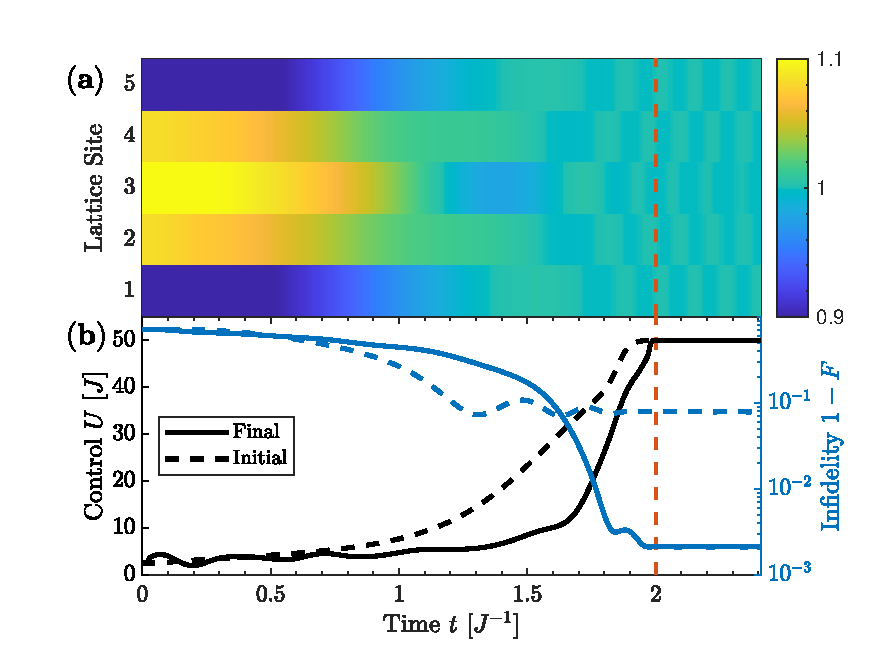
\includegraphics[width=0.9\textwidth]{Figures/L5/RampPlot.pdf}
    \caption{Solution with highest fidelity achieved for duration $T = 2 J^{-1}$ using the interior point method. The dashed, red line marks the end of the duration $T$, after which the system is further evolved according to the final control value. \textbf{(a)} Expectation value of the number operator, $\braket{\hat{n}_i}$, for each site of the lattice during optimal ramp sequence. The coloraxis has been rescaled to show small fluctuations. \textbf{(b)} Initial and optimized ramp sequences along with the corresponding evolution of fidelities.}
    \label{fig:ExtendedRamp}
\end{figure} 

In figure \ref{fig:ExtendedRamp5}(a) the expectation value of the number operator is plotted for each site during the ramp. Initially the system is in the superfluid phase, whereby the its energy is minimized by de-localizing the particles across the lattice. Due to the open boundary conditions, particles can only tunnel in one direction at the outer sites, which effectively causes a depletion of population. 
As the system is evolved towards the Mott-Insulating state, having multiple particles at the same sites becomes very energetically unfavorable. Hence, the target state has approximately only a single particle at each site, where any deviations are due to a finite value of $J/U$.
The optimized ramp brings the system very close to the target configuration of particles, which can be observed near the dashed red line marking the end of the duration, $T$. Some imperfections are present, although their magnitude is exaggerated by the logarithmic color axis.
After the duration of the optimized control sequence the system is further evolved according to $U(T)$. During this additional evolution, oscillations in the population are clearly visible. These oscillations can be attributed to two things: First, if the final state is not the ground state of $\hat{H}(U(T))$, then the system will not be in equilibrium. Therefore, the non-equilibrium dynamics will persist after the control duration. As the final infidelity is around $I(T) \sim 2 \cdot 10^{-3}$, the final state has small deviations from the ground state, whereby this explanation is the most likely. 
Secondly, the oscillations may be due to number fluctuations frozen in by the Kibble-Zurek mechanism. However, the Kibble-Zurek mechanism should be more prominent at longer time scales, when the critical point is crossed slowly. Nevertheless, it may partly be causing the visible oscillations in population.

Meanwhile, in figure \ref{fig:ExtendedRamp5}(b) the initial and optimized control is plotted together with their resulting infidelities. Optimizing the initial seed utilizing the interior point method has resulted in a reduction of almost two magnitudes in obtained infidelity.
While the initial ramp is fairly smooth, the optimized ramp wiggles a bit during the first three quarters of the duration followed by a sharp upswing towards the final control value. The steep increase in the control towards the end is very similar to the adiabatic-like ramp sequence proposed in \cite{Zakrzewski2009}. However, the initial oscillating behavior is highly non-adiabatic, as its oscillations appear to cross the critical point at $(U/J)_{\mathrm{crit}} = 3.37$ multiple times. It should be noted, that this value of the critical point was computed in the thermodynamic limit, whereby it is most likely slightly different for a finite sized system. However, crossing the critical point multiple times may cause interference of generated excitations, essentially creating a shortcut towards the target state. 
In fact, optimized ramp sequences for shorter durations had oscillations with even larger amplitude. Meanwhile, for long durations the solutions could reach a high fidelity through a more adiabatic-like ramp shape.


\subsection{Control Basis Size}
Unlike GRAPE, which takes the full optimization space into account, the chopped basis parameterization employed in GROUP results in a much smaller dimension of the optimization space. The chopped basis does not necessarily span the entire solution space, almost it may be sufficient for the representation of the optimal solution. However, if the chosen basis size is too small, artificial minima may be introduced to the control landscape due to the incompleteness of the basis \cite{Rach2015}. 
The chopped basis employed for both the interior point and Nelder-Mead calculation contain basis functions of the form $f_n = \sin \left( \omega_n t / T \right)$, where $\omega_n = n \pi$ are a set of increasing frequencies.
To investigate the basis size required to describe the optimal solutions, a series of optimizations were made for various basis sizes for the duration $T = 2 J^{-1}$. 
\begin{figure}[h!]
    \centering
    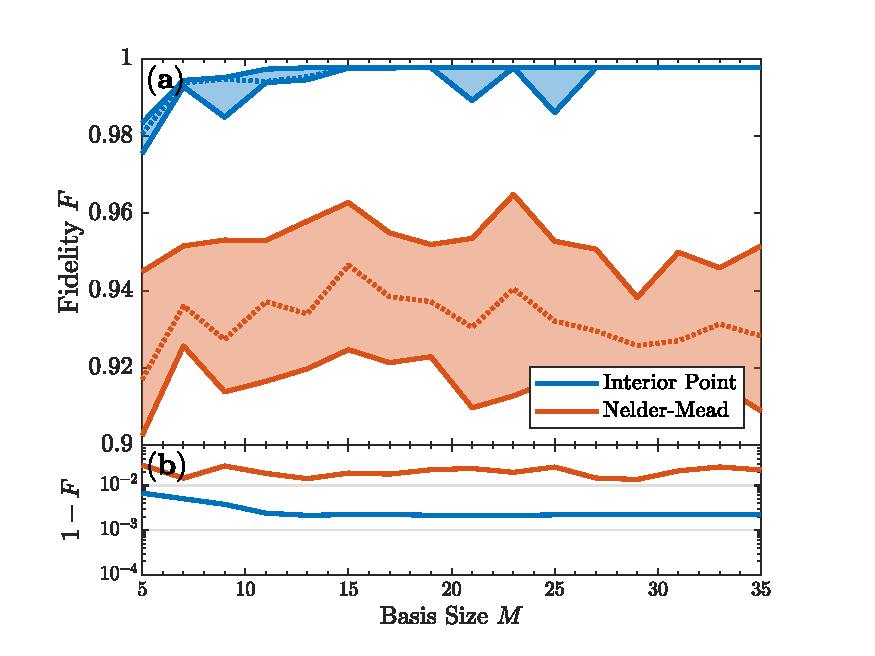
\includegraphics[width=0.9\textwidth]{Figures/L5/FidelityBasisSize.pdf}
    \caption{Final fidelity obtained for optimal control at various chopped basis sizes, $M$, for duration $T = 2 J^{-1}$. \textbf{(a)} The dotted line marks the median fidelity achieved, while the shaded area displays the $25\%$- and $75\%$-quartiles of the solutions. \textbf{(b)} The lowest infidelities achieved for each basis size.}
    \label{fig:FidelityBasisSize}
\end{figure}

The results of a scan over the chopped basis size, $M$, can be seen in figure \ref{fig:FidelityBasisSize}. The calculations were repeated 50 times for each basis size. Starting with the interior point method, the algorithm consistently finds good solutions for basis sizes larger than 15. Although their are a few exceptions, these lower fidelities are likely due to the algorithm getting stuck in local minima already present in the landscape. For $M < 15$ the variance in obtained fidelity clearly increases, which most likely is due to the introduction of artificial minima to the landscape. In figure \ref{fig:FidelityBasisSize}(b) the infidelity of the best solutions at each basis size is displayed. Here, the best solutions for the interior point method start to worsen around $M \sim 11$. The discrepancy in basis size between when the best solution and when the overall solutions become worse is causes by the fact that the optimal may still be realizable using only a few frequencies. Meanwhile, lowering the basis size will introduce an increasing number of artificial minima, until not even the optimal solution is spanned by the basis.
Meanwhile, the Nelder-Mead method produces very varying results, which can be attributed to the algorithm rather than the chopped basis size. While the solutions do appear to become worse for low values of $M$, the inconsistency of the algorithm makes it hard to draw a conclusion on the appropriate basis size. An investigation of a different control problem showed the final fidelity becoming worse for large basis sizes when employing the Nelder-Mead method, as the algorithm struggles optimizing too many parameters at once \cite{sorensen2018}. However, at the basis sizes investigated here, no such phenomenon is apparent.


\section{Application on Larger Systems} \label{sec:appLargeSystems}

The framework already contains all the components required for applications on larger systems, however, in larger the systems the effects of the open boundaries of the lattice is much smaller, whereby a much higher entanglement entropy is expected. Therefore, optimization of larger systems is infeasible employing the very low degree of truncation used for the smaller system. 

When applying the same settings to a system of 15 sites the optimization became increasingly slow for longer durations. Since no maximum bond dimension was specified, the matrices of the tensor network continued to grow in size, as entanglement built up in the system following the phase transition. As the cost of applying the tDMRG propagator scales quadratically with the bond dimension of the state, the time-evolution became increasingly slow. Furthermore, the GRAPE algorithm stores the state at each time step to efficiently compute the gradient, which causes the program to run out of available memory in certain cases. Thus, an analysis of the growth of entanglement within the system is necessary, if the framework is to be applied to larger systems.\\

Further improvements to the convergence rate may be achieved by calculating the Hessian of the cost function. For the purpose of this thesis, the Hessian was approximate using the L-BFGS algorithm, however, this approximation only becomes sufficiently accurate after multiple iterations. Since interior point methods solve a series of subproblems for decreasing barrier heights, the L-BFGS approximation must be restarted multiple times thus reducing its effectiveness \cite{Wachter2006}. On the other hand, supplying interior point methods with analytically derived gradient should result in superlinear convergence \cite{wright}.

A full derivation of the general GRAPE Hessian is presented in Appendix \ref{chap:Hessian} along with the altered version for the Suzuki-Trotter propagator. If both the forward propagated initial state and the backwards propagated target state is kept at each time step, the computation of the Hessian requires an additional $N(N - 1)/2$ step propagations, where $N$ is the total number of time steps of the ramp duration. However, these propagations can be separated into $N$ parallel calculations, which should significantly reduce the computational time of the Hessian. Note, that storing the backwards propagated target state would result in a doubling of the required memory occupied by the algorithm. Therefore, a suitable truncation of the tensor bond dimensions is required for the implementation of the Hessian.

In addition to increasing the convergence rate, valuable information regarding the optimization landscape can be extracted from the Hessian \cite{Shen2006}. Therefore, the addition of the Hessian to the framework may be a necessary step towards application on large systems, however, its implementation is outside the scope of this thesis.


\subsection{Spreading of Correlations and Entanglement}
Truncations of the matrix product state are necessary when optimizing control sequences for large systems, however, the truncation effectively creates a low-entanglement representation of the system. Hence, understanding the growth of entanglement within the system is crucial for the application on larger system. Furthermore, correlations within the system are essential to characterizing the system, whereby studying their evolution versus that of the entanglement entropy will provide valuable insight into the underlying dynamics of the system.

For this study a Bose-Hubbard system of 20 sites and particles was chosen. In a 20-site system, the overall effects of the open boundaries are much smaller, whereby the dynamics in this system are comparable to those of even larger lattices.
Previous studies have shown that the ramping speed greatly affects the dynamics of the system \cite{Lauchli2008,Braun2015}. Therefore, two very different ramps from $U(0) = 2.5 J$ to $U(T) = 50 J$ were examined: An abrupt quench to the final vale, and an exponential ramp typical from experimental procedures. Both ramps lasted a duration of $T = 3 J^{-1}$ and utilized Trotter steps of size $\Delta t = 5 \cdot 10^{-3} J^{-1}$. Furthermore, the maximum occupation at a single sites was limited to 7 bosons, which is relatively high and therefore should not affect the results \cite{Braun2015}. The analysis was carried out using a high truncation threshold of $\epsilon_t = 10^{-8}$ and a maximum bond dimension of $D = 1000$, whereby the entropy was barely limited.\\
\begin{figure}[h!]
    \centering
    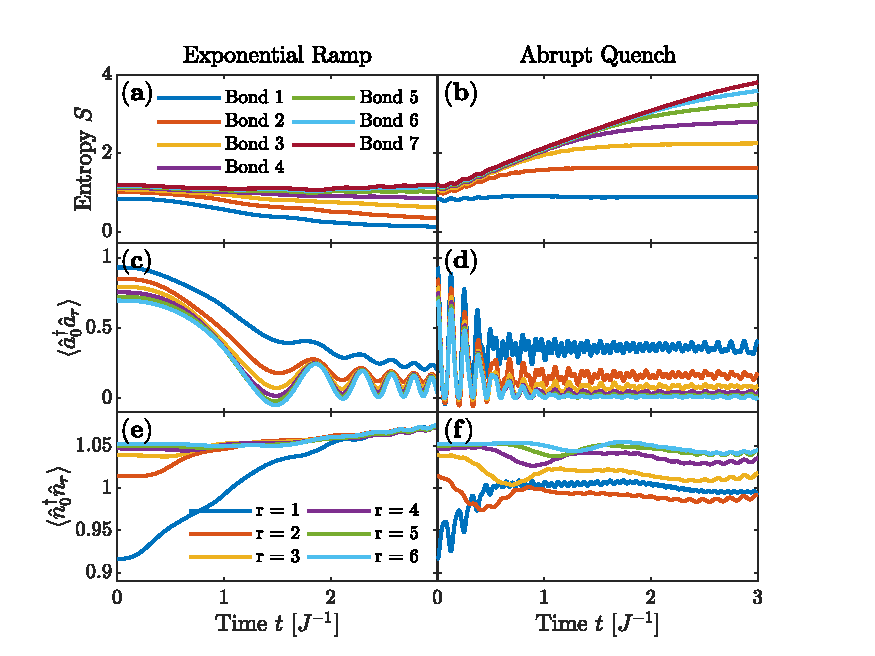
\includegraphics[width=\textwidth]{Figures/L20/EntanglementGrowth.pdf}
    \caption{Dynamical evolution of entanglement entropy and correlations during different types of ramps from $U(0) = 2.5 J$ to $U(T) = 50 J$. \textbf{(a-b)} von-Neumann entropy \eqref{eq:vNEntropy} for bipartitions of the lattice at various bonds, with bond 1 being between lattice sites 1 and 2 and so on. \textbf{(c-d)} Single-particle correlations for different distances $r$. \textbf{(e-f)} Rescaled density-density correlations for different distances $r$.}
    \label{fig:EntanglementGrowth}
\end{figure}

Figures \ref{fig:EntanglementGrowth}(a-b) display the von-Neumann entropy \eqref{eq:vNEntropy} for bipartitions of the lattice at different bonds.
In the case of the exponential ramp, the entanglement entropy between approximately equal sized blocks of the lattice remains almost constant throughout the entire duration. In fact, the entropy across the outer bonds decreases a relatively large amount. Near a critical point, the correlation length and entanglement should diverge for an equilibrium state \cite{Zurek2005}. However, since the system crosses the phase transition dynamically, the ground state decays into a linear combination of excited states, whereby the divergent behavior of the entropy is avoided. Since the exponential ramp is rather slow, it can be considered adiabatic for parts of the duration, whereby no excitations and entanglement is generated. For such a ramp, the dynamics will be influenced by the Kibble-Zurek mechanism \cite{Braun2015}.

On the contrary, the sudden quench in the interaction strength causes a rapid increase of entanglement. Quench dynamics are limited by the Lieb-Robinson bounds \eqref{eq:LiebRobinsonBound}, which is apparent from linear increase in entanglement with slope independent of the block size, $l$.  The saturation value of the entropy depends linearly on the block size, which effectively defines a maximum entropy propagation velocity $v_e$. A linear growth of entropy up to times $t = l/2 v_e$ has been shown for different models \cite{Lauchli2008,Eisert2006,Amico2008,Calabrese2005}, confirming that the spreading velocity is limited by a universal bound. A similar study the Bose-Hubbard model on a 32-site lattice \cite{Lauchli2008} yielded very similar results, whereby the dynamics appear relatively independent of system size.
Thus, the quantum state during a slow ramp can be accurately represented using only a small bond dimension. Meanwhile, a high bond dimension is required to fully describe the rapidly increasing entropy during a fast ramp sequence. \\

Next, the single-particle correlations, $\braket{\hat{a}_{0}^{\dag} \hat{a}_{r}}(t)$, during the two ramps were examined. For comparison it is worth looking at the equilibrium correlations and density matrices previously shown in figure \ref{fig:DensityMatrices}. In equilibrium one observes very long-ranged correlations in the superfluid phase, while the correlations decay exponentially for the Mott-insulation state. Figures \ref{fig:EntanglementGrowth}(c-d) display the single-particle correlations during the ramp sequence for various distances, $r$, from a reference site. Here, the 7th site of the lattice was chosen as reference to avoid the effects of the boundaries of the lattice.
Considering the exponential ramp first, the correlations decrease for the first half of the duration followed by a series of damped oscillations. Around the critical point, the Kibble-Zurek mechanism suggests a decay of correlation length following a power law \cite{Zurek2005}. While this is not entirely obvious from figure \ref{fig:EntanglementGrowth}(c), the correlation length clearly decreases during the first third of the duration, after which it starts growing again. The second half of the sweep duration features large oscillations in the correlations. The Kibble-Zurek mechanism is responsible for freezing in fluctuations, although the superfluid to Mott-transition should predominantly feature number fluctuation. A study of the phase transition via an exponential ramp showed that one would observe Gaussian damped revivals of the phase coherence \cite{Schutzhold2006}. The Gaussian decay should be independent of the distance $r$, which appears to be the case in figure \ref{fig:EntanglementGrowth}(c), as the fluctuations decay relatively similar.

Compared to the exponential ramp, the single-particle correlations behave much more violently, when the system is quenched. Initially, the correlations oscillate with a period of $T_{osc} \approx 2 \pi / U(T)$. These oscillations originate from the spectrum of the interaction part of the Bose-Hubbard Hamiltonian. Consider the case of negligible tunneling, whereby the evolution of the single-particle correlations is
\begin{equation}
	\braket{\hat{a}_{i}^{\dag} \hat{a}_{j}}(t) = \sum_{ \{ n \} , \{ n' \}} c_{n}^{*} c_{n'} \Braket{ \{ n \} | \hat{a}_{i}^{\dag} \hat{a}_{j} | \{ n' \}} \; \delta_{n_i , n_{i}' +1} \; \delta_{n_j , n_{j}' -1} \; e^{i U(T) (n_j ' - n_i ' - 1) t} \; ,
	\label{eq:CorrelationEvolution}
\end{equation}
where $\{ n \}$ is the set of Fock states with $n_i$ particles on the $i$'th site, and $c_n$ are coefficients of a general state \cite{Lauchli2008}. Only Fock state pairs corresponding to a particle begin annihilated at site $j$ and created at site $i$ will contribute to $\Braket{ \{ n \} | \hat{a}_{i}^{\dag} \hat{a}_{j} | \{ n' \}}$. As a result, the frequencies of the time evolution are given by $U(T) (n_j ' - n_i ' - 1)$. For a Mott-insulator with unit occupation all sites are populated equally, whereby the corresponding frequency is $-U(T)$ yielding an oscillation period $T_{osc} = 2 \pi / U(T)$. However, when starting in a superfluid state, the number fluctuations will result in frequencies containing higher multiplies of $U(f)$. Thus, the amplitude of higher-order frequencies is determined by the starting value $U(0)$.
In this case, the initial value is rather close to the critical point, whereby higher-order frequencies are not apparent until the first-order frequency has decayed sufficiently. At $t \approx 0.5 J^{-1}$ a beat-like structure in the oscillations is visible signifying contributions from higher-order frequencies. 
The single-particle correlation evolution \eqref{eq:CorrelationEvolution} assumes a vanishing tunneling. However, any finite tunneling will cause a spread in the frequencies, which ultimately leads to the decay of the oscillations in time \cite{Kollath2007}. Such decaying revivals have been observed experimentally in a Bose-Hubbard system \cite{Greiner2002collapse}.

After the relaxation of the oscillations, the system reaches a quasi-steady state with only minor fluctuations. These residual fluctuation in the correlations can be interpreted as number fluctuations of the superfluid being "frozen in" during the quench. As these number-fluctuations may be long-lived \cite{Schutzhold2006}, the residual oscillations remain for longer times. 

Clearly, neither the exponential ramp nor the quench produces an equilibrium Mott-insulator, as the final state has large, oscillating correlation functions. Nevertheless, while not being a Mott-insulator, the quenched system reaches a quasi-steady state. An investigation of the problem in \cite{Kollath2007} revealed that the steady-state correlation lengths were determined mainly by the difference between the initial and quenched value of $U$. Thus, the final state could be categorized as belonging to one of two non-equilibrium phases: A \textit{non-thermal steady state} produced by a large quench, and a \textit{thermalized state} for smaller quenches. The state obtained here is distinctly non-thermal, as it retains a strong memory of its initial state.\\

Finally, the evolution of density-density correlations, $\braket{\hat{n}_{0}^{\dag} \hat{n}_{r}}(t)$, was investigated, as shown in figures \ref{fig:EntanglementGrowth}(e-f). Since the number operator, $\hat{n}_i$, commute with the interaction term of the Bose-Hubbard Hamiltonian, no large oscillations should be present in the strong coupling limit. For the case of the exponential ramp this is indeed the case, as the correlations at all distances decay towards the same constant value associated with equal population across the lattice. For a perfect Mott-insulator and unit occupancy the density-density correlations should converge to 1. However, as established earlier, the exponential ramp clearly does not produce the ground state Mott-insulator, whereby the deviations are expected. Interestingly, small oscillations in the correlations are present at later times for all distances. This is most likely caused by the superfluid number-fluctuations frozen in by the Kibble-Zurek mechanism.

When quenching the system, the density-density correlations behave much differently. Due to rapid change of the interactions, the correlations can no longer relax into a common value but are instead almost frozen in from the start. At short distances, the correlations appear increasingly Mott-like, while at longer ranges the large variances in population becomes apparent. Further examining the first half of the quench duration, it is clear that some signal is propagating through the system at what appears to be a constant velocity.
\begin{figure}[h!]
    \centering
    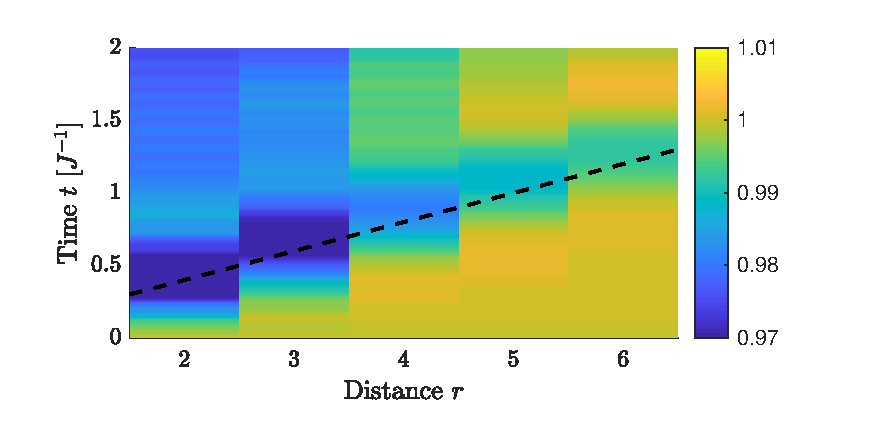
\includegraphics[width=0.8\textwidth]{Figures/L20/CorrelationLightCone.pdf}
    \caption{Time evolution of normalized density-density correlations $\braket{\hat{n}_{0}^{\dag} \hat{n}_{r}}(t) / \braket{\hat{n}_{0}^{\dag} \hat{n}_{r}}(0)$ after an abrupt quench. The correlations are spreading with a constant velocity, and the front of the evolution is marked by a dashed line.}
    \label{fig:CorrelationLightCone}
\end{figure}
Plotting the evolution of the density-density correlations as a function of distance produces figure \ref{fig:CorrelationLightCone}, where the light-cone-like propagation of correlations is very obvious. For distances $r >  v_c t$, with $v_c$ being the propagation velocity of correlation, the correlations are constant, despite the system having already undergone the quench. In the limit of very fast ramps (where a quench is instantaneous), the propagation of correlations can be interpreted as ballistically spreading quasi-particles \cite{Cheneau2012,Calabrese2006}. The propagation velocity of the correlations is bounded by the Lieb-Robinson bound \ref{eq:LiebRobinsonBound}, resulting in the effective light-cone. An even clearer light-cone was shown in \cite{Lauchli2008} by rescaling the correlations accordingly.\\

The exponential ramp and the quench represent two limits of ramping speeds. The exponential ramp is slow, whereby the system can react almost adiabatically, as no violent oscillations in the correlations are present. Nevertheless, the product of exponential ramp is clearly not a perfect Mott-insulator, as correlation functions point towards number fluctuations in the final state. However, since the entanglement entropy of the system does not increase during the ramp, the tensor network description of the state is very accurate at even long timescales.
On the other hand, the dynamics of the correlations following a quench are much more violent, as the ramp is essentially instantaneous. At long timescales, the system starts to reach a steady-state, although this state appears non-thermal from its correlations, whereby it has very different characteristics than the Mott. An optimal ramp will most likely contain elements from both fast and slow ramps in order to produce a high-fidelity Mott-insulator at a low ramp duration. 



\subsection{Required Bond Dimension for Non-Equilibrium Dynamics}
The main limiting factor when performing quantum optimal control is the computational cost of the time-evolution. Thus, for large systems it is vital to maintain a minimal bond dimension during the entire ramp duration. The previous analysis illustrated the dynamics of a 20 site system with unit occupation during a fast and a slow ramp. Here, the effect of truncating the tensors at various maximum bond dimension is investigated. As an exponential ramp causes no increase in the entanglement entropy of the system, the system should be much easier to simulate. Therefore, it is of interest just how few contributing eigenstates need to kept in order to produce a final state comparable to a non-truncated one.
For this analysis, an even slower, $T = 5 J^{-1}$, exponential ramp was used. The truncation threshold was kept at $\epsilon_t = 10^{-8}$, while the maximum bond dimension was varied. The calculation was carried out for Trotter step-sizes of $\Delta t = 5 \cdot 10^{-3} J^{-1}$ and $\Delta t = 10^{-2} J^{-1}$ and produced similar results. Here the results for a step size of $\Delta t = 10^{-2} J^{-1}$ are shown, as this step size is more likely to be used for the optimization of a larger system.\\ 

\begin{figure}[h!]
    \centering
    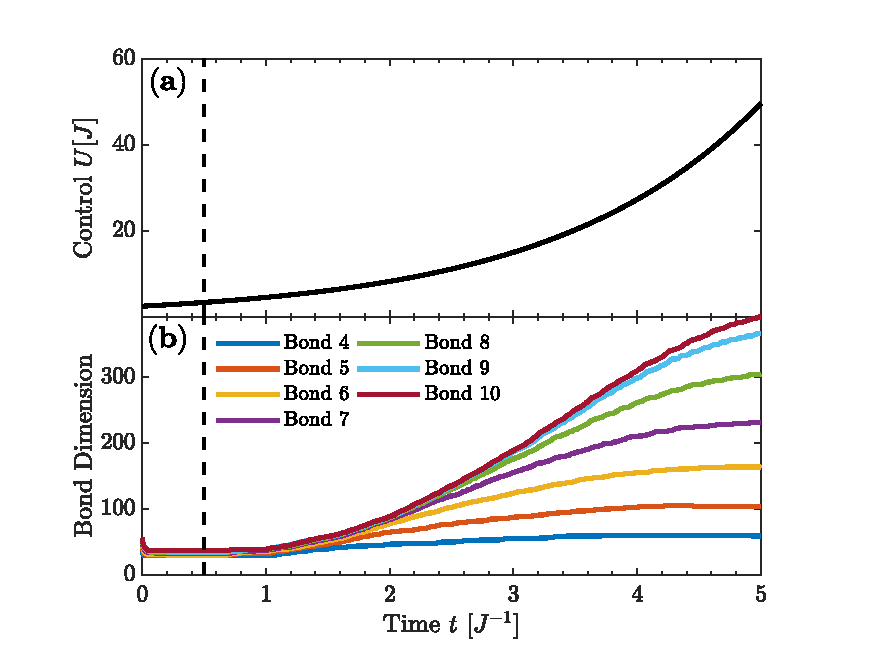
\includegraphics[width=0.9\textwidth]{Figures/L20/BondDimEvolution.pdf}
    \caption{ Evolution of bond dimensions during an exponential ramp. \textbf{(a)} The exponential ramp from $U(0) = 2.5 J$ to $U(T) = 50 J$. The crossing of the critical point is marked by the dashed line. \textbf{(b)} Dimension of various bonds of the matrix product representation of the quantum state. }
    \label{fig:BondDimEvolution}
\end{figure}
First, the growth of bond dimension during the ramp was investigated, which is shown in figure \ref{fig:BondDimEvolution}. In subfigure (a) the exponential ramp is shown, and the time at which it crosses the critical point is marked by a dashed line. The bond dimensions of the initial superfluid state evolved according to the ramp is displayed in figure \ref{fig:BondDimEvolution}(b). Initially, the bond dimension remains constant, which is expected from the previous results showing the entanglement entropy decreasing during the ramp duration. However, a short while after having crossed the critical point, the dimension of all inner bonds starts increasingly rapidly. This increase in bond dimension is very similar to the increase in entropy following a sudden quench, however, it is most unexpected in the case of the exponential ramp. Although the bond dimension of a matrix product state is expected to increase as it is time evolved \cite{Daley2004}, the truncation threshold of $\epsilon_t = 10^{-8}$ should maintain a low bond dimension throughout the duration.
\begin{figure}[h!]
    \centering
    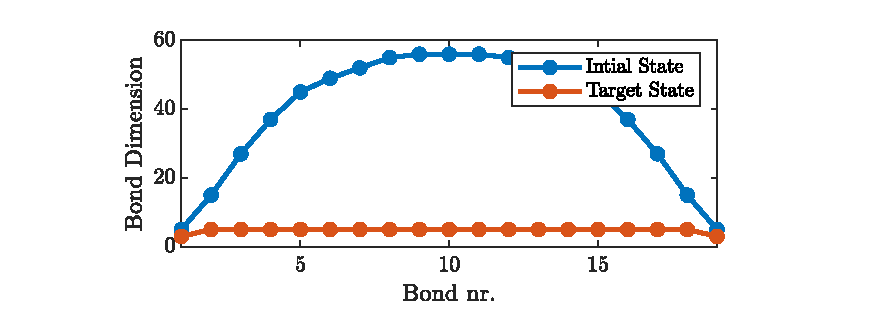
\includegraphics[width=0.9\textwidth]{Figures/L20/InitialBondDim.pdf}
    \caption{ Bond dimensions of the initial superfluid ground state for $U = 2.5 J $ and the target Mott-insulating ground state for $U = 50 J $.}
    \label{fig:InitialBondDim}
\end{figure}
For comparison, the bond dimensions of the initial and target states are illustrated in figure \ref{fig:InitialBondDim}. The superfluid ground state has long-ranged correlations resulting in a parabola-like distribution of bond dimensions. Meanwhile, the exponentially decaying correlations of the ground state Mott-insulator causes a flat distribution of bond dimensions, and the state is well represented using only very few eigenstates. Thus, the matrix product representation of the evolved state is very different from the ground state. However, when examining the entanglement and correlations following the exponential ramp in figure \ref{eq:CorrelationEvolution}, the high bond dimension seem redundant for the description of the state. Therefore, dynamically truncating the matrices at a low maximum bond dimension, $D$, should not alter the dynamics of the system considerably.

\begin{figure}[h!]
    \centering
    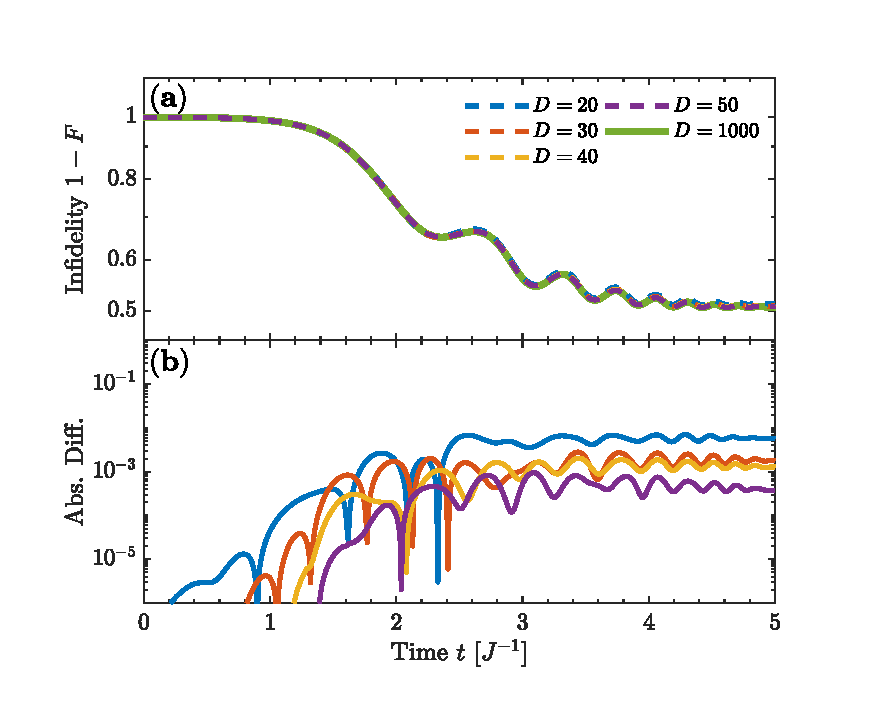
\includegraphics[width=0.9\textwidth]{Figures/L20/FidelityTruncation.pdf}
    \caption{ \textbf{(a)} Obtained infidelity with regards to the Mott-insulating ground state for the exponential ramp. The calculation was carried out for different maximum bond dimension $D$. \textbf{(b)} Absolute difference between infidelities obtained with no truncation ($D = 1000$) and those employing a maximum bond dimension.  }
    \label{fig:FidelityTruncation}
\end{figure}
To prove that the bond dimension of the evolved state is artificially high, the same initial state was evolved according to the same exponential ramp while begin truncated at a given maximal bond dimension, $D$. The results shown in figure \ref{fig:FidelityTruncation} reveal that the obtained infidelity barely changes when decimating the bond dimension. While a weak scaling with maximum bond dimension was expected \cite{Daley2004}, the amount of redundant information in the $D = 1000$ evolution is still surprising. According to figure \ref{fig:FidelityTruncation}(b), choosing a maximal bond dimension of $D = 30$ should produce a difference in infidelity a magnitude smaller than the threshold for the quantum speed limit. Meanwhile, the time evolution of the truncated state should proceed much faster, as the application of the propagator scaled quadratically with the bond dimension.

\begin{figure}[h!]
    \centering
    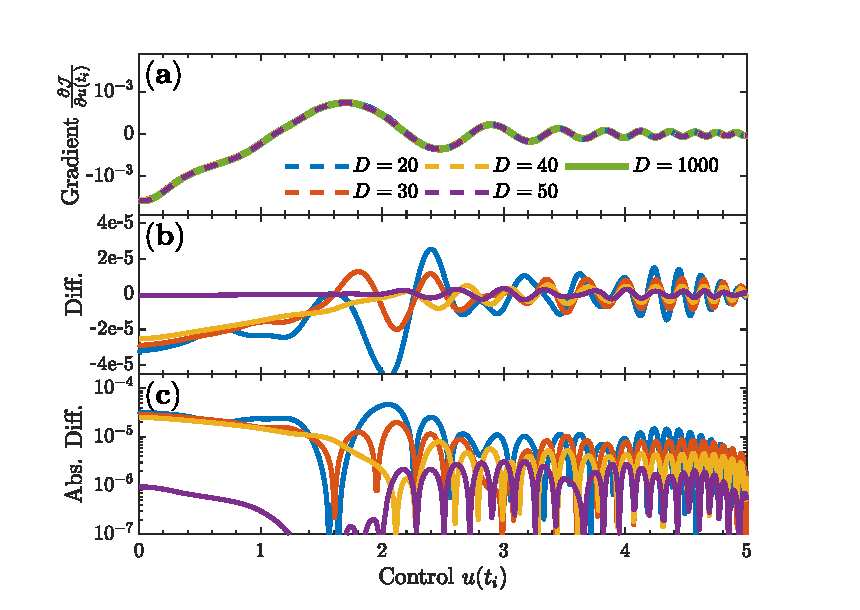
\includegraphics[width=0.9\textwidth]{Figures/L20/GradientTruncation.pdf}
    \caption{ \textbf{(a)} Gradient elements of the cost function \ref{eq:STcostgrad} for the exponential ramp. The calculation was carried out for different maximum bond dimension $D$. \textbf{(b)} Difference in gradient element between the non-truncated state ($D = 1000$) and the states having a maximum bond dimension. \textbf{(c)} Absolute value of the differences. }
    \label{fig:GradientTruncation}
\end{figure}
Lastly, it is also worth examining how the truncation affects the gradient elements, as having accurate derivatives is essential for a fast convergence rate \cite{deFouquieres2011}. Figure \ref{fig:GradientTruncation} shows the results of calculating the gradient elements \ref{eq:STcostgrad} for the exponential ramp without any regularization. Compared with the infidelity, the gradient scales more strongly with the maximum bond dimension. Therefore, the truncation is limited by the derivative of the cost function rather than the function itself. Unlike the infidelity, the gradient becomes gradually better during the ramp sequence. The same phenomenon is discussed in section \ref{sec:TrotterGrad} and is caused by the accumulated error when calculating $\ket{\chi (0)}$. 
While the bond dimensions of the matrix product state start growing rapidly after crossing the critical point, neither the infidelity nor the gradient show no signs of being influenced by the phase transition whatsoever. This discrepancy remains open for interpretation, however, it points towards optical control methods being well suited for studying phase transitions. 